\section{Implementation}
To combine SLP with our group key agreement protocol we changed/added following protocol properties:
\begin{itemize}
  \item SLP message
  \item Key enchantment
  \item Communication
\end{itemize}

\subsection{SecuredSLP message format}
The header of a SLP message was modified to distinguish SLP messages from SecuredSLP messages. We added the \texttt{S}, \texttt{Security Group Length} and \texttt{Security Group Name} flags into the header and changed the \texttt{Version} of SLP in the source code (compare figure \ref{fig:slp-header} and figure \ref{fig:sslp-header}).
\begin{description}
\item[Version:] Is now set to 3.
\item[S:] This flag shows that the message body is encrypted.
\item[Security Group Length:] This flag specifies the length of the \texttt{Security Group Name} string.  
\item[Securety Group Name:] This flag shows the name of the security group the message belongs to.
\end{description}

\begin{figure}[!h]
\begin{lstlisting}
	 0                   1                   2                   3
	 0 1 2 3 4 5 6 7 8 9 0 1 2 3 4 5 6 7 8 9 0 1 2 3 4 5 6 7 8 9 0 1
	+-+-+-+-+-+-+-+-+-+-+-+-+-+-+-+-+-+-+-+-+-+-+-+-+-+-+-+-+-+-+-+-+
	|    Version    |  Function-ID  |            Length             |
	+-+-+-+-+-+-+-+-+-+-+-+-+-+-+-+-+-+-+-+-+-+-+-+-+-+-+-+-+-+-+-+-+
	| Length, contd.|O|F|R|       reserved          |Next Ext Offset|
	+-+-+-+-+-+-+-+-+-+-+-+-+-+-+-+-+-+-+-+-+-+-+-+-+-+-+-+-+-+-+-+-+
	| Next Extension Offset, contd. |              XID              |
	+-+-+-+-+-+-+-+-+-+-+-+-+-+-+-+-+-+-+-+-+-+-+-+-+-+-+-+-+-+-+-+-+
	|      Language Tag Length      |         Language Tag          |
	+-+-+-+-+-+-+-+-+-+-+-+-+-+-+-+-+-+-+-+-+-+-+-+-+-+-+-+-+-+-+-+-+
\end{lstlisting}
\label{fig:slp-header}
\caption{SLPv2 Header}
\end{figure}

\begin{figure}[!h]
\begin{lstlisting}
	 0                   1                   2                   3
	 0 1 2 3 4 5 6 7 8 9 0 1 2 3 4 5 6 7 8 9 0 1 2 3 4 5 6 7 8 9 0 1
	+-+-+-+-+-+-+-+-+-+-+-+-+-+-+-+-+-+-+-+-+-+-+-+-+-+-+-+-+-+-+-+-+
	|    Version    |  Function-ID  |            Length             |
	+-+-+-+-+-+-+-+-+-+-+-+-+-+-+-+-+-+-+-+-+-+-+-+-+-+-+-+-+-+-+-+-+
	| Length, contd.|O|F|R|S|     reserved          |Next Ext Offset|
	+-+-+-+-+-+-+-+-+-+-+-+-+-+-+-+-+-+-+-+-+-+-+-+-+-+-+-+-+-+-+-+-+
	| Next Extension Offset, contd. |              XID              |
	+-+-+-+-+-+-+-+-+-+-+-+-+-+-+-+-+-+-+-+-+-+-+-+-+-+-+-+-+-+-+-+-+
	|      Language Tag Length      |         Language Tag          |
	+-+-+-+-+-+-+-+-+-+-+-+-+-+-+-+-+-+-+-+-+-+-+-+-+-+-+-+-+-+-+-+-+
	|      Security Group Length    |      Security Group Name      |
	+-+-+-+-+-+-+-+-+-+-+-+-+-+-+-+-+-+-+-+-+-+-+-+-+-+-+-+-+-+-+-+-+
\end{lstlisting}
\label{fig:sslp-header}
\caption{SecuredSLP Header}
\end{figure}
Additionally we use a HMAC (96 Bit) over the header and add it into the encrypted message body so the header and payload are linked with each other. This method is also used in IPSec under the ESP mode and allows us to prevent replay attacks and header manipulation of each SecuredSLP message. See also \textcolor{red}{quellen nachher einf�gen}

\subsection{Key enchantment in SecuredSLP}\label{sec:keyenchange}
Like discussed above we use a group key agreement protocol to establish security between group members. To get knowledge about a security group, clients use extra discovery iteration. The information about a security group is announced as plain text; otherwise no one would be able to join such a group. To join a security group a user has to send a join message to the group. Then the group key agreement protocol handles the key distribution. In our implementation we used TGDH, so the distribution works like discussed in section \ref{sec:TGDH}. After receiving the group key, security group members are able to discover services which are pronounced in this security group or provide services themselves. Also there is a rekeying phase after a user leaves the group. That is important to keep the security under the group members and to avoid that a key gets compromised.

\subsection{Communication in SecuredSLP}
Due to the additional changes in the protocol it is necessary to take a look at the communication between network members. SecuredSLP still provides unencrypted communication like in SLPv2 so it is still possible to create or join a unsafe SLP scope. In that case the communication works like in SLPv2 (compare section \ref{sec:intro}) without a group agreement protocol. In case SecuredSLP tries to establish connection to a security group the communication can be described as following:
\begin{enumerate}
  \item User discovers a security group and sends a \textit{JoinMessage} to the group key agreement protocol (TGDH in our case)
  \item Group key agreement protocol initializes the rekeying phase for the security group and computes new group key.
  \item New member receives the group key and is able to communicate with the other security group members. Compare with figure \ref{fig:sslp_join}
\end{enumerate}
\begin{figure}[!h]
\centering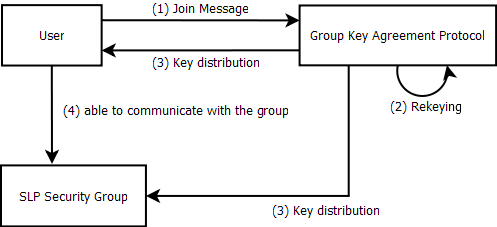
\includegraphics[width=0.5\textwidth]{Images/sSLP_join}
\label{fig:sslp_join}
\caption{Communication sequence of a user joining a SecuredSLP security group}
\end{figure}
Like told above the group agreement protocol is just a module adjacent to SLP and works asynchronous with it. Hence the key distribution is more complicated and fault-prone. Also there is just one valid key in the network at time so most problems arrive if a rekeying phase is initialize and there are still messages in the network encrypted with the old group key. Those messages will be refused by SecuredSLP.